\documentclass[zavrsnirad]{fer}
% Dodaj opciju upload za generiranje konačne verzije koja se učitava na FERWeb
% Add the option upload to generate the final version which is uploaded to FERWeb


\usepackage{blindtext}
\usepackage{xcolor}
\usepackage{listings}

\lstset{ %
	language=Python,
	basicstyle=\ttfamily\footnotesize,
	keywordstyle=\color{blue},
	commentstyle=\color{green},
	stringstyle=\color{red},
	showstringspaces=false,
	frame=single,
	numbers=left,
	numberstyle=\tiny\color{gray},
	breaklines=true,
	breakatwhitespace=true,
	tabsize=2
}

\usepackage[labelfont=bf]{caption}

\usepackage{changepage} % For adjusting margins
\usepackage{multirow}

%--- PODACI O RADU / THESIS INFORMATION ----------------------------------------

% Naslov na engleskom jeziku / Title in English
\title{Optical character recognition system for older books in Croatian}

% Naslov na hrvatskom jeziku / Title in Croatian
\naslov{SUSTAV ZA OPTIČKO RASPOZNAVANJE TEKSTA STARIJIH KNJIGA NA HRVATSKOME JEZIKU}

% Broj rada / Thesis number
\brojrada{1605}

% Autor / Author
\author{Dominik Agejev}

% Mentor 
\mentor{Prof.\@ Tomislav Hrkać}

% Datum rada na engleskom jeziku / Date in English
\date{September, 2024}

% Datum rada na hrvatskom jeziku / Date in Croatian
\datum{rujan, 2024.}

%-------------------------------------------------------------------------------


\begin{document}


% Naslovnica se automatski generira / Titlepage is automatically generated
\maketitle


%--- ZADATAK / THESIS ASSIGNMENT -----------------------------------------------

% Zadatak se ubacuje iz vanjske datoteke / Thesis assignment is included from external file
% Upiši ime PDF datoteke preuzete s FERWeb-a / Enter the filename of the PDF downloaded from FERWeb
\zadatak{hr_0036537505_73.pdf}


%--- ZAHVALE / ACKNOWLEDGMENT --------------------------------------------------

\begin{zahvale}
  % Ovdje upišite zahvale / Write in the acknowledgment
  Jakovu, Lovri i Roku,
  hvala na pomoći!
\end{zahvale}


% Odovud započinje numeriranje stranica / Page numbering starts from here
\mainmatter


% Sadržaj se automatski generira / Table of contents is automatically generated
\tableofcontents


%--- UVOD / INTRODUCTION -------------------------------------------------------
\chapter{Uvod}
\label{pog:uvod}

Cilj rada nadići je uspješnost gotovih sustava za optičko raspoznavanje teksta (eng. \textit{Optical Character Recognition} ili \textit{OCR}) na starijim knjigama hrvatskoga jezika koristeći se nenadziranim metodama učenja, odnosno bez označenih podataka za trening modela, uz predobradu i naknadnu obradu.

Iako suvremeni sustavi poput DTrOCR-a \cite{Fujitake2023} postižu gotovo savršene rezultate u raznim primjenama, optičko raspoznavanje teksta  nipošto nije riješen problem. Još uvijek i najbolji sustavi, poput gore navedenog, pogrešno prepoznaju više od 10\% riječi na fotografijama teksta „u divljini“ i gotovo 20\% riječi u rukopisima na kineskom jeziku.

Uz to, zbog ovisnosti o jezičnim modelima, novija rješenja općenito nisu primjenjiva bez dodatne prilagodbe na manje zastupljene jezike, poput hrvatskog, ili se pak oslanjaju na veliku količinu označenih podataka ili na sintetičke podatke, generirane modelima koji za rjeđe jezike nisu dostupni, te zahtijevaju značajne računalne resurse.

Nadalje, zbog suviše uske primjene, specifični problemi, poput predmeta ovog rada, raspoznavanja teksta antikvarnih knjiga i to na jeziku ograničene uporabe, redovito se zaobilaze u prilog doprinosima aktualnim primjenama. \cite{Olejniczak2022}

U okviru ovog rada najprije se uvodi u područje, metode i temeljne pojmove koji će se koristiti u radu. Zatim je detaljno izložen zadatak i njegove specifičnosti uz pregled dosadašnjih postignuća unutar područja.

Prelazeći na izvedbu rješenja, razmatraju se najznačajniji slobodno dostupni OCR alati prikladni zadatku, a to su Tesseract \cite{Smith2007}, OCR sustav opće namjene koji održava Google, te Ocular \cite{Berg-Kirkpatrick2013}, razvijen specifično za primjenu na antikvarnim dokumentima.

Nakon treniranja i optimiziranja hiperparametara Oculara, uspoređen je s Tesseractom na već predobrađenim ispitnim podacima gdje se pokazuje da usprkos starijoj arhitekturi u bitnome nadjačava Tesseract, ali uz određena ograničenja.

Konačno, izveden je sustav glasanja kojim se postiže veća uspješnost od one samostalnih modela.


%	\begin{figure}[htb]
%	  \centering
%	  \includegraphics[width=0.38\linewidth]{Figures/lenovo_yoga_tab3_pro_front.png} 
%	  \caption{Moja prva slika}
%	  \label{slk:prvaslika}
%	\end{figure}

% Referenciramo se na sliku \ref{slk:prvaslika} u sredini rečenice, zatim prije zareza \ref{slk:prvaslika}, te zatim na kraju rečenice \ref{slk:prvaslika}.
% Upravo smo testirali radi li naredba \verb|\ref| ispravno u slučaju kada nakon nje slijedi točka.


%-------------------------------------------------------------------------------
\chapter{Uvod u OCR}
\label{pog:ocr_uvod}

Optičko raspoznavanje teksta grana je računalnog vida koja se bavi izdvajanjem teksta iz slika, bilo dokumenata, rukopisa ili scenskih fotografija, radi lakog pretraživanja i uređivanja, jednostavnijeg arhiviranja ili pak dostupnosti sadržaja slabovidnima i slijepima.

U odnosu na sadržaj ulaznih slika najčešće govorimo o prepoznavanju teksta tiskanih dokumenata, rukopisa ili teksta „u divljini“, npr. natpisa na pročeljima trgovina, s tim da je potonje uže povezano s drugim granama računalnog vida poput detekcije i klasifikacije objekata.

OCR sustavi često se razvijaju i za još uže definirane zadatke, primjerice prepoznavanje teksta na računima ili antikvarnim dokumentima. Takvi sustavi, kakvima se bavi i ovaj rad, nazivaju se jednonamjenskima (eng. \textit{task-specific}), dok se sustavi prilagođeni raznim uporabama zovu sustavima opće namjene (eng. \textit{general purpose}). \cite{Borovikov2014}

Optičko raspoznavanje teksta podrazumijeva u bitnome pet koraka: predobradu, segmentaciju, izdvajanje značajki, klasifikaciju te naknadnu obradu. \cite{Dhande2017} U ovom poglavlju izložit će se ugrubo najznačajnije metode i pojmovi koji će se koristiti u ostatku rada.

\section{Predobrada}

Predobrada se odnosi na postupak prilagodbe ulazne slike radi uspješnijeg raspoznavanja znakova. Načela po kojima se ravna predobrada uključuju pojednostavljenje ulaza izostavljanjem nebitnih informacija, što čine binarizacija i eliminacija šuma, te ispravljanje fizičkih nesavršenosti, uzrokovanih bilo tiskom bilo digitalizacijom ulaza, što rade metode poput ispravljanja nagnuća (eng. \textit{skew correction}).

\subsection{Binarizacija}
\label{Binarizacija}

Cilj binarizacije razlučivanje je između teksta i pozadine. Najjednostavniji način za to postavljanje je praga (eng. \textit{thresholding}) za koji su svi pikseli s RGB ili sivotonskim (eng. \textit{grayscale}) vrijednostima nižim od praga obojani crno, tj. označeni kao tekst, a pikseli iznad praga označeni kao pozadina. \cite{Jyotsna2016}

Razlikujemo globalne i lokalne metode binarizacije. Globalne, poput često korištene Otsuove  metode \cite{Otsu1979}, postavljaju jedan prag za cijeli dokument, što je vremenski učinkovito i uspješno u idealnom slučaju s jednoličnom pozadinom, no zakazuje pri nejednakom osvjetljenju ili sjeni uslijed loše skeniranog pregiba knjige. Lokalne, poput metode adaptivnog kontrasta \cite{Su2013}, temeljenoj na prepoznavanju rubova pomoću kontrasta susjednih piksela, nešto su resursno zahtjevnije, ali zato daju bolje rezultate. \cite{Otsu1979, Su2013}

\subsection{Ispravljanje nagnuća}

Cilj ispravljanja nagnuća zaokrenuti je retke teksta tako da su vodoravni. Utvrđivanje kuta nagnuća redaka binarizirane slike može se svesti na pronalazak pravca koji najbolje aproksimira redak, a u tu svrhu najčešće se koristi Houghova transformacija. \cite{Hassanein2015} Konceptualno, Houghova transformacija za svaku rubnu točku slike pronalazi parametre (m, c) pravaca koji se kroz nju mogu provući. Pronađeni skup parametara zapravo je pravac u m, c prostoru, a odredivši pripadajući pravac svakoj točci, ako neki pravci imaju zajedničko sjecište, kroz njima pripadne točke moguće je povući pravac koji u konkretnom slučaju određuje redak teksta.

\section{Segmentacija}

\section{Izdvajanje značajki}

Starije metode OCR-a, prije prelaska na neuronske mreže, koristile su ručno definirane značajke (poput tzv. Granlundovih opisnika temeljenih na Fourierovoj transformaciji) \cite{Trier1996} dok u suvremenim sustavima poput Tesseracta raniji slojevi neuronske mreže izdvajaju značajke

\section{Klasifikacijske arhitekture}

\subsection{Usporedba predložaka}

\subsection{CNN}

\subsection{RNN}

\subsection{LSTM}

\textit{long short-term memory} (\textit{LSTM})

\section{Naknadna obrada}

\textcolor{red}{\textit{Tesseract zamjena ',,' (dva zareza) s " (ravni navodnici)}}

%-------------------------------------------------------------------------------
\chapter{OCR starijih tekstova}
\label{pog:ocr_starijih_tekstova}

Iz specifičnosti zadatka, tj. starosti knjiga,  proizlaze određene poteškoće, naime:
\begin{itemize}
	\item Čest višak ili manjak tinte pri tisku pojedinih znakova
	\item \textcolor{red}{Zastarjela znakovlja (fontovi) s neuobičajenim znakovima} %(npr. ſ , ʒ )
	\item Otežana predobrada zbog spremanja na mikrofilmu
	\item Arhaičan jezik
	\item Neravan tisak
	\item Istrošenost i oštećenja papira
\end{itemize}



\section{Pregled literature}

\cite{Berg2013}
\cite{Springmann2014}
\cite{Christy2017}
\cite{Wick2018}
\cite{Garrette2015}
\cite{Garrette2016}


%-------------------------------------------------------------------------------
\chapter{Tesseract}
\label{pog:tesseract}

Tesseract \cite{Smith2007} je najpoznatiji i najprecizniji slobodno dostupan OCR sustav opće namjene koji podržava i hrvatski jezik, a od 4. inačice temeljen je na LSTM neuronskim mrežama. U ovom poglavlju objasnit će se ugrubo Tesseractov proces prepoznavanja teksta prema zadanim postavkama.

\section{Predobrada}

Tesseract ima ugrađena tri koraka predobrade: binarizaciju, eliminaciju šuma i analizu uređenja stranica.

\subsection{Binarizacija}

Tesseract se koristi Otsuovom metodom, no ne za postavljanje jednog globalnog praga za čitavu stranicu, već rabi implementaciju Leptonica biblioteke \cite{Leptonica} koja dijeli stranicu u jednake blokove te na njima postavlja prag. Takvim pristupom nadvladavaju se varijacije u svjetlini na makro razini slike, ali se zadržava i veća resursna učinkovitost uslijed paralelizacije i izbjegavanja složenijih računa lokalnih metoda.

Za slike koje nisu više-manje dvobojne nego pate od većih nejednakosti u osvijetljenju Tesseract podržava i Sauvolinu \cite{Sauvola1997} lokalnu metodu binarizacije koja utvrđuje prag za svaki piksel slike na temelju srednje vrijednosti i standardne devijacije okolnih piksela.

\subsection{Eliminacija šuma}

Razlučivši pozadinu od ostatka prelazi se na brisanje šuma poput razlivene tinte. To se postiže pronalaskom spojenih piksela te usporedbom karakteristika nakupine s tipičnim karakteristikama teksta.

Tijekom analize razmatra se: \cite{Tesseract}

\begin{description}
	\item[Širina poteza] \hfill \\ Potezi jednolične širine vjerojatnije pripadaju znaku.
	\item[Veličina nakupina] \hfill \\ Skupine piksela koje se protežu izvan uobičajene visine retka vjerojatno nisu znakovi.
	\item[Obujmljena površina] \hfill \\ Gledajući površinu koju skupina piksela okružuje možemo procijeniti je li znak ili nije.
	\item[Broj nakupina po retku] \hfill \\ Brojeći skupine piksela u retku provjerava se omjer malih nakupina naspram skupina veličine znaka.
 	\item[Odnos među točkama] \hfill \\ Ako se detektira velik broj susjednih točaka na istoj visini ne odbacuju se već su označene kao "vodeće točke" sadržaja.
\end{description}

\subsection{Analiza uređenja stranice}

\begin{description}
	\item[Detekcija slika] \hfill \\ Funkcijom \texttt{FindImages} Tesseract pronalazi slike koje potom zanemaruje prilikom prepoznavanja teksta.
	\item[Detekcija crta] \hfill \\ Tesseract rabi Leptonicu za pronalaženje i uklanjanje crta, odnosno razdjelnih linija, na ulaznoj slici što pomaže u odvajanju teksta od grafičkih elemenata poput tablica ili obrazaca.
	\item[Analiza povezanih komponenti] \hfill \\ Ovaj korak izvodi funkcija \texttt{find\_components} koja skenira binarnu sliku piksel po piksel, označava povezane crne piksele i grupira ih u povezane komponente koje predstavljaju potencijalne znakove ili dijelove znakova.
	\item[Detekcija orijentacije i pisma] \hfill \\ Ako je ova opcija omogućena, Tesseract će provjeriti o kojem je pismu riječ (latinično, kinesko, ...) i u kojem smjeru se piše (kineski se npr. može pisati odozgo prema dolje ili zdesna na lijevo).
	\item[Detekcija stupaca] \hfill \\ Koristi se ako je tekst pisan u stupcima poput novinskog članka ili znanstvenog rada.
	\item[Pronalazak redaka teksta] \hfill \\ Tesseract analizira prostorne odnose između povezanih komponenti kako bi detektirao linije teksta. Ovaj korak koristi statistički pristup temeljen na razmacima između komponenti.
\end{description}

\section{Klasifikacija}

\section{Naknadna obrada}

\cite{Breuel2013} o LSTM-u


%-------------------------------------------------------------------------------
\chapter{Ocular}
\label{pog:ocular}

Ocular \cite{Berg2013} je sustav za optičko raspoznavanje teksta razvijena specifično za rad s povijesnim dokumentima, i koji je, kada je izdan i svojevremeno unaprjeđen \cite{Berg2014}, bio vrhunac tehnologije za to područje (eng. \textit{state-of-the-art}).

Njegove glavne značajke su: \cite{Ocular}

\begin{itemize}
	\item Nenadzirano učenje nepoznatih znakovlja rabeći slike ulaznog dokumenta i korpus teksta na ciljnom jeziku.
	\item Prilagođenost radu sa šumovitim dokumentima.
	\item Podrška za višejezične dokumente.
	\item Nenadzirano učenje ortografskih varijacija uslijed arhaičnog pravopisa.
	\item Istovremen ispis doslovnog teksta i normaliziranog oblika (prilagođenog standardnom jezku).
\end{itemize}

%-------------------------------------------------------------------------------
\chapter{Metodologija}
\label{pog:metodologija}

Ključan dio razvoja boljeg rješenja evaluacija je preciznosti Tesseracta i Oculara. U tu svrhu potreban je ispitni skup podataka prilagođen ograničenjima sustava. 

Zatim treba prikupiti podatke za treniranje Oculara i namjestiti njegove hiperparametre da daju zadovoljavajuće rezultate, što će zapravo biti najznačajniji dio rada.


\section{Ispitni skup podataka}

Budući da Tesseract ima ugrađenu predobradu slika, radi pravednije usporedbe same klasifikacije teksta izabrani su već obrađeni dokumenti:

\begin{itemize}
	\item Fra Jozo Garić, biskup – Korizmena okružnica (1932.)
	\item Sv. Petar Kanizije – Summa nauka christianskoga (1583.)
\end{itemize}

Korizmena okružnica korištena je za većinu ispitivanja, a \textit{Summa} je izabrana za isprobavanje ortografskih mogućnosti te kao primjer teškog ulaza za sustav.

\begin{figure}[h!]
	\centering
	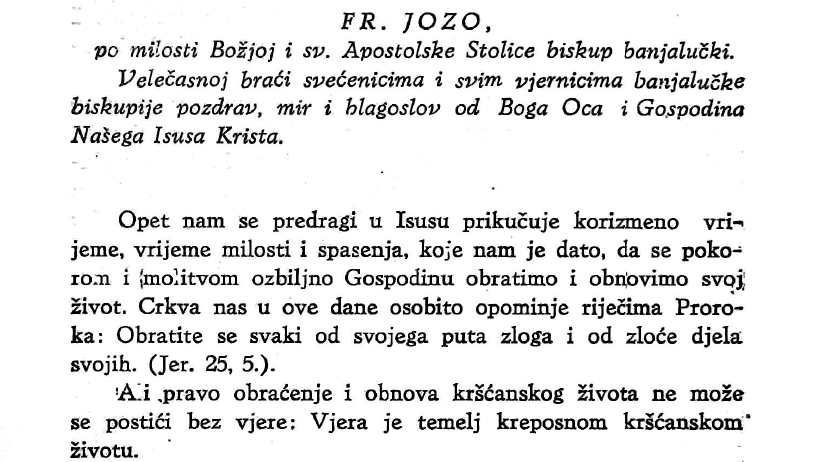
\includegraphics[width=1.0\linewidth]{Figures/korizmena.png} 
	\caption{Izvadak iz \textit{Korizmene okružnice}}
	\label{slk:korizmena}
\end{figure}

\begin{figure}[h!]
	\centering
	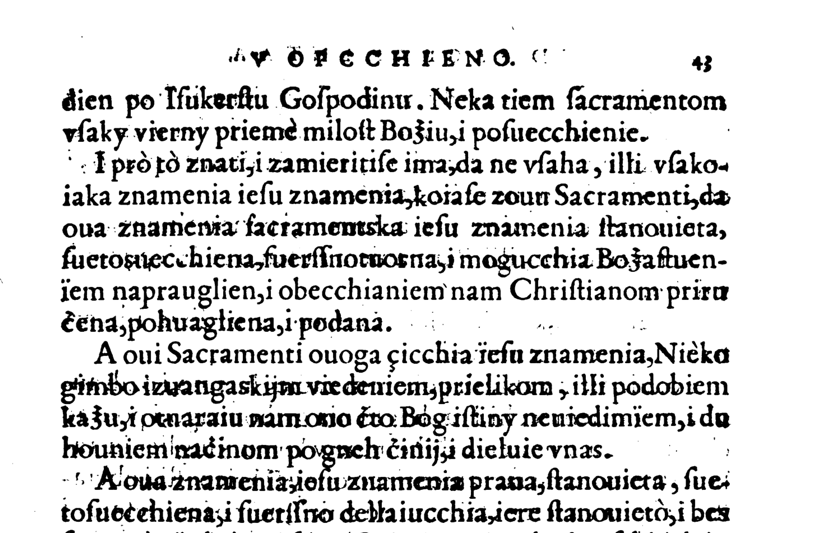
\includegraphics[width=1.0\linewidth]{Figures/summa.png} 
	\caption{Izvadak iz \textit{Summe nauka christianskoga}}
	\label{slk:summa}
\end{figure}

Oba sustava imaju određena ograničenja na ulaze: 

Ocular radi jedino s PDF dokumentima zastarjele verzije 1.4 te ih je stoga bilo potrebno pretvoriti u taj format. Za to je korišten Ghostscript, \cite{Ghostscript} slobodno dostupan alat otvorenog koda. 

Tesseract pak radi jedino na slikama te je zato bilo potrebno ekstrahirati ih iz PDF-a prije prepoznavanje teksta. Ovdje je zgodno napomenuti da treba paziti da se prilikom pretvorbe ne smanji DPI rezolucija jer to ima poguban utjecaj na preciznost.

\section{Mjere uspješnosti}

Za uspoređivanje znakovnih nizova najčešće korištena mjera uspješnosti je \textbf{Levenshteinova udaljenost} koja bilježi broj potrebnih zamjena, brisanja ili umetanja znakova da bi se iz jednog niza dobio drugi. \cite{Levenshtein1965}

Budući da ta mjera ovisi o duljini teksta, dijeljenjem Levenshteinove udaljenosti ukupnim brojem znakova dobivamo \textbf{stopu pogreške za znakove} (eng. \textit{Character Error Rate}). Obično se dobrom vrijednošću smatra 1-2\%.

\textbf{Stopa pogreške za riječi} (eng. \textit{Word Error Rate}) dobiva se uzimanjem riječi za najmanju jedinicu zamjene pri računanju Levenshteinove udaljenosti, tj. ako su jedan ili više znakova u riječi pogrešni čitava riječ broji se kao pogrešna, te dijeljenjem te udaljenosti s ukupnim brojem riječi.


\subsection{F1?}

\subsection{Recall?}


%-------------------------------------------------------------------------------
\chapter{Optimizacija Oculara}
\label{pog:optimizacija_oculara}

Za razliku od Tesseracta, Ocular nije univerzalno primjenjiv za različite jezike i znakovlja već je potrebno naučiti jezični model, za koji je potreban korpus teksta na ciljnom jeziku, te model fonta, koji se gradi na temelju slika čiji će tekst kasnije prepoznavati.

\section{Jezični model}

Pri izgradnji skupa podataka za trening jezičnog modela najrelevantnije su dvije stavke: broj podataka i tematika teksta.

U izvornom radu pokazano je kako model malo precizniji (4 WER postotna boda) na dokumentima čija je tematika pokrivena u jezičnom modelu. Budući da je sustav namijenjen starijim knjigama, od kojih je dobar dio vjerske tematike, uključeno je Sveto Pismo i druge duhovne knjige pored novijeg i starijeg štiva koje doprinosi većoj raznolikosti izričaja i opsežnijem rječniku.
\cite{Berg2013}

U daljnjim eksperimentima korišten je jezični model treniran na tekstovima javno dostupnih knjiga, poput djela Augusta Šenoe, Marije Jurić-Zagorke, Charlesa Dickensa i sl. (7.5 milijuna riječi) uz Šarićev prijevod Svetog Pisma (670k riječi) i još 11 knjiga vjerske tematike (500k riječi). 

Ukupan broj riječi odabranog skupa podataka od 8.7 milijuna usporediv je sa skupom podataka korištenim u izvornom radu koji ih ima 10 milijuna.

\subsection{Veličina skupa podataka}

Ispitani su i podskupi odabranog ali i veći skupovi podataka, temeljeni na prethodno navedenom uz dva tipa proširenja: stranom i domaćom beletristikom (11.6 milijuna riječi) te tekstovima vjerske tematike (6 milijuna riječi).

Tekstovi vjerskih knjiga nisu bili lektorirani nego nesavršeni proizvodi prepoznavanja teksta, a uključeni su svejedno kako bi se ispitalo doprinosi li kvantiteta potencijalno više od kvalitete ako greške nisu značajne.

Moglo bi se očekivati da će veći rječnik više doprinijeti uspjehu na tekstovima s dotad manjom preciznošću prepoznavanja, kao što je \textit{Summa nauka christianskoga}, međutim, ni smanjenje ni povećanje skupa podataka nije dovelo do poboljšanja u preciznosti, a proširenje je značajno usporilo trening i transkripciju.

\bgroup
\def\arraystretch{1.25}
\begin{table}[h]
	\centering
	\begin{tabular}{|c|c|c|c|}
		\hline
		\textbf{Ispitivani dokument} & \textbf{Jezični model} & \textbf{CER} & \textbf{WER} \\ \hline
		Korizmena okružnica & Izvorni & 1.06 & 2.76 \\ \hline
		Korizmena okružnica & Izvorni + OCR vjerskih knjiga & 1.59 & 3.64 \\ \hline
		Summa nauka christianskoga & Izvorni & 25.41 & 68.71 \\ \hline
		Summa nauka christianskoga & Izvorni + OCR vjerskih knjiga & 24.05 & 65.99 \\ \hline
	\end{tabular}
	\caption{Usporedba uspješnosti jezičnih modela}
	\label{tab:lm_performance}
\end{table}
\egroup

Minimalno poboljšanje vidljivo u tablici \ref{tab:lm_performance} za \textit{Summu} u granicama je slučajnosti, osobito uzevši u obzir da je za tu knjigu ispitivana samo jedna stranica (iako je trening modela fonta bio na 6) naspram 12 za Korizmenu okružnicu.

\subsection{Veličina snopa}

S obzirom na to da veći jezični model podrazumijeva više mogućih kombinacija riječi, povećanje snopa ispitivanih riječi u Markovljevom modelu postaje potencijalno presudno kako bi točna riječ bila pronađena.

Ipak, kako je vidljivo iz donje tablice \ref{tab:7.2}, povećanje snopa nije dovelo do poboljšanja niti pri treningu modela fonta niti prilikom transkripcije.

\bgroup
\def\arraystretch{1.25}
\begin{table}[h]
	\centering
	\begin{tabular}{|c|c|c|c|c|}
		\hline 
		\multicolumn{2}{|c|}{\textbf{Veličina snopa}} & \multicolumn{1}{|c|}{\multirow{2}{*}{\textbf{CER}}} & \multicolumn{1}{|c|}{\multirow{2}{*}{\textbf{WER}}} \\ \cline{1-2}
		
		\textbf{Trening}  & \textbf{Transkripcija}  & \multicolumn{1}{|c|}{}  & \multicolumn{1}{|c|}{}  \\ \hline
		40 & 40 &  1.59 & 3.64   \\ \hline
		40 & 120 & 1.81 & 3.77   \\ \hline
		120 & 50 & 2.21 & 5.04 \\ \hline        
		120 & 120 & 2.29 & 5.78 \\ \hline                                             
	\end{tabular}
	\caption{Usporedba uspješnosti prema veličini snopa}
	\label{tab:7.2}
\end{table}
\egroup

Rezultati impliciraju kako je bolje ne ispraviti prepoznati znakovni niz ako predloženi ispravak nije među prvima predložen. To može biti do grešaka u skupu podataka za jezični model, gdje veći snop obuhvati i rijetke pogrešne, ali slične nizove ispravljanome. 

S druge strane, može biti posljedica inherentnog ograničenja stohastičkog modela. Tomu u prilog ide, primjerice, zamjena rijetkog niza \texttt{vjere:}, koji se vjerojatno nije nalazio u skupu podataka, riječju \texttt{vjetar}. 

\section{Model znakovlja}

Lorem ipsum

\bgroup
\def\arraystretch{1.25}
\begin{table}[h]
	\centering
	\begin{tabular}{|c|c|c|c|c|}
		\hline
		\multirow{2}{*}{\textbf{Iteracije treninga}} & \multicolumn{2}{|c|}{\textbf{Veličina snopa}} & \multicolumn{1}{|c|}{\multirow{2}{*}{\textbf{CER}}} & \multicolumn{1}{|c|}{\multirow{2}{*}{\textbf{WER}}} \\ \cline{2-3}
		
		& \textbf{Trening}  & \textbf{Transkripcija}  & \multicolumn{1}{|c|}{}  & \multicolumn{1}{|c|}{}  \\ \hline
		3x3    & 10    & 10 &  2.03 & 3.58  \\ \hline
		3x3 & 50  & 50 & \textbf{1.06} & \textbf{2.76}   \\ \hline
		3x3+2x2 & 50 & 50 & 1.19 & 2.9 \\ \hline                                              
	\end{tabular}
	\caption{\textcolor{red}{Lorem ipsum}}
	\label{tab:__________}
\end{table}
\egroup

\section{Ispitivanje ortografskih mogućnosti/značajki}


%-------------------------------------------------------------------------------
\chapter{Sinteza rješenja}
\label{pog:sinteza_rješenja}

Budući da je izuzev ispuštanja određenih redaka Ocular točniji od Tesseracta, kako je utvrđeno u prethodnom poglavlju, ovdje predlažemo jednostavan sustav glasanja kojim je Ocularova manjkavost otklonjena bez gubitka preciznosti.

Algoritam glasanja čita redak po redak Tesseractov ispis i traži odgovarajući redak Ocularovog ispisa na temelju sličnosti izračunate pomoću Levenshteinove udaljenosti. Ako pronađe dovoljno sličan redak odabire ga kao izlaz, inače preferira Tesseractov ispis.

\begin{figure}[h]
	\centering
	\begin{adjustwidth}{1cm}{1cm}
		\begin{lstlisting}
			for t_line in tesseract_output:
				for c_line in ocular_output:
					distance = Levenshtein.distance(t_line, c_line)
					if distance < threshold * len(t_line):
						output.append(c_line)
					break
				output.append(t_line)
		\end{lstlisting}
	\end{adjustwidth}
	\caption{Algoritam glasanja predstavljen Python kodom}
	\label{fig:python_code}
\end{figure}

\bgroup
\def\arraystretch{1.25}
\begin{table}[h]
	\centering
	\begin{tabular}{|c|c|c|c|}
		\hline
		\textbf{OCR sustav} & \textbf{Pojedinosti} & \textbf{CER} & \textbf{WER} \\ \hline
		Ocular & & 8.83 & 10.94 \\ \hline
		Ocular & Zanemareni retci s CER>20 & 1.06 & 2.76 \\ \hline
		Tesseract & & 1.52 & 3.77 \\ \hline
		Predložen sustav & & \textbf{0.96} & \textbf{2.48} \\ \hline
	\end{tabular}
	\caption{Uspješnosti sustava}
	\label{tab:system_performance}
\end{table}
\egroup



%-------------------------------------------------------------------------------
\chapter{Diskusija}
\label{pog:diskusija}

Ideje za nadogradnje: počeci i krajevi redaka su obično Ocularu kritični. Tesseract češće prepoznaje interpunkciju kada treba i kada ne treba.

Ograničenja Oculara - brzina, CUDA (java)


%--- ZAKLJUČAK / CONCLUSION ----------------------------------------------------
\chapter{Zaključak}
\label{pog:zakljucak}

Komentirati konvergenciju računalnog vida, neuralnih mreža, NLP-a i OCR-a.



%--- LITERATURA / REFERENCES ---------------------------------------------------
% Literatura se automatski generira iz zadane .bib datoteke / References are automatically generated from the supplied .bib file
% Upiši ime BibTeX datoteke bez .bib nastavka / Enter the name of the BibTeX file without .bib extension
\bibliography{library}



%--- SAŽETAK / ABSTRACT --------------------------------------------------------

% Sažetak na hrvatskom
\begin{sazetak}
  Cilj rada nadići je uspješnost gotovih sustava za optičko raspoznavanje teksta na starijim knjigama hrvatskoga jezika koristeći se nenadziranim metodama učenja, uz predobradu i naknadnu obradu. Razmatraju se najznačajniji slobodno dostupni OCR alati prikladni zadatku, Tesseract, OCR sustav opće namjene koji održava Google, te Ocular, razvijen specifično za primjenu na antikvarnim dokumentima. Nakon treniranja i optimiziranja hiperparametara Oculara, uspoređen je s Tesseractom gdje se pokazuje da usprkos starijoj arhitekturi u bitnome nadjačava Tesseract, ali uz određena ograničenja. Konačno, izveden je sustav glasanja kojim se postiže veća uspješnost od one samostalnih modela.
\end{sazetak}

\begin{kljucnerijeci}
  OCR; optičko raspoznavanje teksta; računalni vid; Ocular; Tesseract;
\end{kljucnerijeci}


% Abstract in English
\begin{abstract}
  The aim of the paper is to surpass the accuracy of out-of-the-box systems at Optical Character Recognition of historical documents in the Croatian language relying on unsupervised learning methods, preprocessing and postprocessing. The most appropriate freely available OCR tools are evaluated, namely Tesseract, a general-purpose OCR system maintained by Google, and Ocular, developed specifically for use on historical documents. After training and optimizing Ocular's hyperparameters it is compared to Tesseract where it is shown that despite its older architecture Ocular in the main still bests Tesseract, with certain caveats. Finally, a voting-based system is implemented which achieves greater success than each model alone.
\end{abstract}

\begin{keywords}
  OCR; Optical Character Recogniton; Computer Vision; Ocular; Tesseract;
\end{keywords}


%--- PRIVITCI / APPENDIX -------------------------------------------------------

% Sva poglavlja koja slijede će biti označena slovom i riječi privitak / All following chapters will be denoted with an appendix and a letter
\backmatter

\chapter{The Code}

\Blindtext


\end{document}
